\documentclass{article}

\usepackage[utf8]{inputenc}
\usepackage[spanish]{babel}
\usepackage{graphicx}
\usepackage{amsmath}

\title{Modelos Matemáticos}
\author{Guadalupe Escobedo}
\begin{document}
\maketitle
\section{Ecuaciones en diferencias}
\subsection{Primer orden}
Sabemos que: $$\lim_{x\to\infty}\frac{1}{x}=0$$

Calcular los valores propios de $$A=
\begin{pmatrix}
1 & 2\\
\pi & 4

\end{pmatrix}.
$$

Tenemos \$1000 que vamos a invertir a un interés del 1\% mensual.

El valor de la inversión cuando han transcurrido $n$ meses es $$x_n=1000(1.01)^n$$.

Una gráfica de resultado es:

\begin{center}
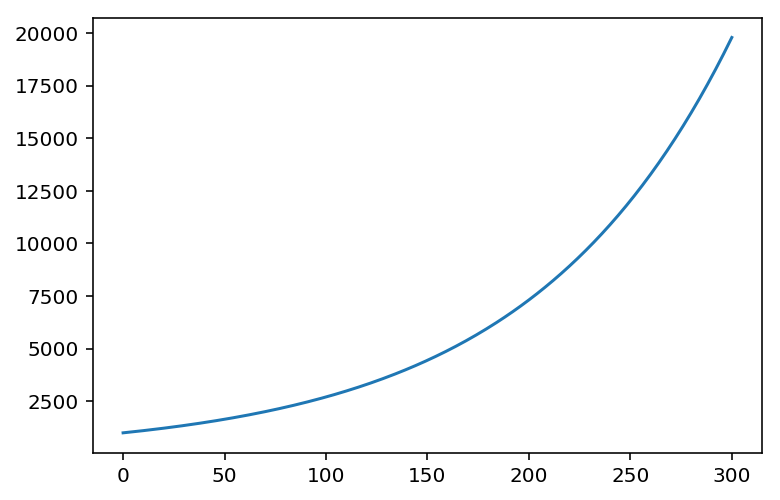
\includegraphics[width=8cm]{grafica}
\end{center}

Para encontrar este resultado, ocupamos que:
$$\sum_{i=0}^{n-1}a^i=\frac{1-a^{n}}{1-a}$$.

La ecuación $x_{n+1}=ax_n+b$ se llama la ecuación en diferencias de primer orden lineal con coeficientes constantes no homogénea.

Algunos valores de la inversion:
\begin{center}
\begin{tabular}{|c|r|}

\hline
Mes & Valor\\ 
\hline
0 & 1000 \\
1 & 1010 \\
2 & 1021.10 \\
3 & 1030.301 \\
\hline
\end{tabular}
\end{center}


\begin{center}
\huge
\textbf{Biomatemáticas}
\end{center}

\subsection{Segundo orden}




\end{document}
